\documentclass[output=paper]{langsci/langscibook} 
\author{Kordula De Kuthy\affiliation{Universität Tübingen}}
\title{Information structure}

% \chapterDOI{} %will be filled in at production

%\epigram{Change epigram in chapters/03.tex or remove it there }
\abstract{Information structure as the hinge between sentence and
  discourse has been at the center of interest for linguists working
  in different areas such as semantics, syntax or prosody for several
  decades. A constraint-based grammar formalism such as HPSG encoding
  multiple levels of linguistic representation within the architecture
  of signs opens up the possibility to elegantly integrate such
  information about discourse properties. In this chapter, we discuss
  a number of approaches that have explored how to best integrate
  information structure as a separate level into the representation of
  signs. We discuss which lexical and phrasal principles have been
  implemented in these approaches and how they constrain the
  distribution of the various information structural
  features. Finally, we discuss how the various approaches are used to
  formulate theories about the interaction of syntax, prosody and
  information structure. In particular, we will see several cases
  where (word order) principles that used to be stipulated in syntax
  can now be formulated as an interaction of syntax and discourse
  properties.  }

\maketitle

\begin{document}
\label{chap-information-structure}



\section{Introduction} 


The \textit{information structure} of a sentence captures how the meaning
expressed by the sentence is integrated into the discourse.
The \textit{information structure} thus encodes which part of an
  utterance is informative in which way, in relation to a particular context.
A wide range of approaches exists with respect to the question what
should be regarded as the primitives of the information structure.

It is now commonly assumed that there are three basic dimensions of
information structure\footnote{For a comprehensive overview of the different research strands with respect to information structural dimension, see \citet{KruijffSteedman2003}.} that are encoded in natural languages and that
have been assumed as the basic primitives: (i) a distinction between
what is new information advancing the discourse (\emph{focus}) and
what is known, i.e., anchoring the sentence in existing (or
presupposed) knowledge or discourse (\emph{background}), (ii) a
distinction between what the utterance is about (\emph{topic},
\emph{theme}) and what the speaker has to say about it
(\emph{comment}, \emph{rheme}), and (iii) a dimension referred to as
\textit{information status} where entities that have already been
mentioned in the discourse (\textit{given}) are distinguished from
those that have not been mentioned (\emph{new}). For all three ways of
partitioning the information structure, we find approaches within the
HPSG framework.  Example (\ref{ex:info-struc}) illustrates, how one
utterance in the context of a question can be structured according to
different partitionings of information structure.
\begin{exe}
\ex\label{ex:info-struc}
\begin{xlist}
\exi{Q:}  What does Sarah drink?
\exi{A:}  \begin{tabular}[c]{|c|c|c|}
\multicolumn{2}{c|}{\small\textsl{background}} & \multicolumn{1}{c}{\small\textsl{focus}}\\\hline 
Sarah & drinks & TEA.\\\hline
\multicolumn{1}{c|}{\small\textsl{topic}} & \multicolumn{2}{c}{\small\textsl{comment}}\\
  \end{tabular}
\end{xlist}

\end{exe}

The focus/background division with focus as the part of an utterance
that is informative with respect to the discourse is one of the most
commonly adopted partitioning when studying information structure, and
thus many approaches within the HPSG architecture as well assume a
division into focus and background, such as the ones that will be
discussed in this article: \cite{EV96a}, \cite{deKuthy2002a},
\cite{Webelhuth2007a-u}, \cite{Paggio2009a-u}, \cite{Bildhauer2008a},
\cite{song-bender:2012} and \cite{song2018}. Less common within the
HPSG framework are approaches that take topic, i.e. the material that
an utterance is about, as the central notion and assume topic and
comment (or theme and rheme) as the primitives of the information
structure. Most approaches discussed here assume that the background
has one designated (mostly referential) element functioning as the
topic (or link), among them are \cite{EV96a}, \cite{deKuthy2002a},
\cite{Paggio2009a-u}, and \cite{song2018}.

With respect to information status (including primitives such as new and
given mentioned above) the discourse status of referential elements is of
interest, i.e. whether they can be linked to previously mentioned
items, i.e. whether they are (discourse) old or given, or whether they
haven't been mentioned before and are thus (discourse) new. The
representation of information status has received comparatively little
interest within the HPSG community, the approach by
\cite{DeKuthy.Meurers-11} is one of the few approaches that
explicitly integrate this dimension into their information structural
architecture.

The need to represent discourse properties in a grammar architecture
of signs results from the insight that in many, if not all, languages
the way utterances are realized via their syntactic structure,
morphological patterns and prosody very often interacts with discourse
requirements of these utterances. In other words, approaches dealing
with constraints on word order in a particular construction need to
encode that this particular word order is only grammatical given a
particular context, or a particular accent pattern has to be connected
to a particular discourse status of the accented elements.\footnote{For some examples in the literature where this has been explored for word order phenomena, see for example \cite{ambridge.goldberg-08,DeKuthy.Konietzko-19,Culicover.Winkler-19}. }
Most of the approaches discussed here deal with such interface
questions, and we therefore discuss the particular word order and
phonetic theories that have been implemented in Sections \ref{sec:word-order}
and \ref{sec:prosody} in detail. As a starting point, however, we will first
discuss the various architectural designs that have been implemented in
order to be able to formulate the specific theories integrating
discourse constraints.

\section{Information structure in the architecture of signs}

Several ways of representing information structure within the
architecture of signs have been pursued as part of the HPSG framework:
one of the earliest approaches, which is similar to the idea of
F-marking as pursued in many syntax-based approaches to information
structure in \isi{Generative Grammar} \citep[such
as][]{Jackendoff72a-u, Selkirk84a-u},
%Alternativ dazu ginge auch (such as \citealt{Jackendoff72a-u,Selkirk84a-u})
has been proposed by \cite{Mandahar94a-u}. He assumes that all signs
have an additional appropriate feature \textsc{info"=struc} which
takes as its value objects of the sort \textit{info-type}. A sign can
then have one of the subtypes of \textit{info-type} shown in
\pref{fig:manand-info-struc} as its informational marking.
\ea \label{fig:manand-info-struc}
Type hierarchy under \textit{info-type} of \cite{Mandahar94a-u}:
        \textit{
           \begin{forest}
             [info-type
                [focus]
                [background
                     [link]
                     [tail]
                ]
             ]
           \end{forest}}
\z

% \begin{figure}[htb!]
%   \begin{center}
%         \textit{
%            \begin{forest}
%              [info-type
%                 [focus]
%                 [background
%                      [link]
%                      [tail]
%                 ]
%              ]
%            \end{forest}}
%     \caption{Type hierarchy under \textit{info-type} of \cite{Mandahar94a-u}}
%     \label{fig:manand-info-struc}
%   \end{center}
% \end{figure}

The distribution of the \textsc{info"=struc} values in a sign is determined by
the \isi{\textit{Focus Inheritance Principle}}, which enforces that in every
phrase, the \textsc{info"=struc} value of the mother subsumes the values
of the \textsc{info"=struc} of all of its daughters. The consequence of
this principle is that if one daughter in a phrase is in the focus and
the other one in the ground, then the mother's \textsc{info"=struc} value is the
smallest common super-type of both, namely \textit{info-type}.

There are two problematic aspects of such an architecture. Firstly, it
leads to a proliferation of syntactic markup of non-syntactic
properties, in particular once one considers the full range of
information structure notions, such as focus and focus projection,
multiple foci, and the marking of other discourse functions such as
topic. And secondly, the perspective of information structure as
resulting from an independent interpretation process of syntactic
markup does not support a view of syntax, information structure, and
intonation as directly interacting modules, a view that can be nicely
implemented in a multi-layer framework such as HPSG.
More common are thus approaches that encode the information structure
as a separate layer, i.e., a feature with its own structural
representation.

In the original setup of signs introduced in \cite{ps2}, the feature
\textsc{context} is introduced as part of \textit{local} objects as a
place to encode information relating to the pragmatic context (and
other pragmatic properties) of utterances. In \cite{EV96a} it is
argued that it would be most natural to also represent information
structural information as part of this \textsc{context}
feature. \cite{EV96a} thus introduce the feature \textsc{info"=struc}
as part of the \textsc{context} and since they couch their
approach into Vallduv{\'{\i}}'s \citeyear{vallduvi:92} information packaging account,
\textsc{info"=struc} is further divided into \textsc{focus} and
\textsc{ground}. All \textsc{info"=struc} features take entire signs as
their values. The complete specification is shown in
\pref{fig:e-v-info-struc}.
\ea \label{fig:e-v-info-struc}
Information structure in \cite[56]{EV96a}
        \leavevmode
    \begin{avm}
    [\tp{sign}\\
     synsem|local|context|info-struc & [focus & sign\\
                                        ground & [link & sign\\
                                                  tail & sign]
                                       ]
    ]     
    \end{avm}
\z
% \begin{figure}[htb!]
%   \begin{center}
%         \leavevmode
%     \begin{avm}
%     [\tp{sign}\\
%      synsem|local|context|info-struc & [focus & sign\\
%                                         ground & [link & sign\\
%                                                   tail & sign]
%                                        ]
%     ]     
%     \end{avm}
%     \caption{Information structure in \cite{EV96a}}
%     \label{fig:e-v-info-struc}
%   \end{center}
% \end{figure}

Another approach locating the representation of information structure
within the \textsc{context} feature is the one by
\cite{Paggio2009a-u} as part of a grammar of \ili{Danish}. The
\textsc{infostr} features \textsc{topic}, \textsc{focus} and
\textsc{bg} take as their values lists of indices. Since
\cite{Paggio2009a-u} includes Minimal Recursion Semantics (MRS,
\citealt{CFPS2005a}) as the semantic representation\footnote{A detailed
  discussion of the properties and principles of MRS as implemented in
  HPSG can be found in \crossrefchaptert{semantics}.}, these indices
can be structure shared with the argument indices of the semantic
relations collected on the \textsc{rels} list of the content of a
sign. The basic setup is illustrated in \pref{fig:paggio-infostr}.
% \begin{figure}[htb]
%   \centering
%         \leavevmode
%     \begin{avm}
%     [\tp{sign}\\
%      synsem|local|context|infostr & [focus & list-of-indices\\
%                                      topic & list-fo-indices\\
%                                      bg & list-of-indices]
%     ]     
%     \end{avm}
%   \caption{Information structure in \cite{Paggio2009a-u}}
%   \label{fig:paggio-infostr}
% \end{figure}

\ea\label{fig:paggio-infostr}
Information structure in \cite[149]{Paggio2009a-u}:\\
        \leavevmode
    \begin{avm}
    [\tp{sign}\\
     synsem|local|context|infostr & [focus & list-of-indices\\
                                     topic & list-fo-indices\\
                                     bg & list-of-indices]
    ]     
    \end{avm}
\z

Several approaches encode information structure as part of the \textsc{content},
such as \cite{song2018} and \cite{song-bender:2012}. Since they also
use MRS as the semantic representation language, they enrich the
architecture of \textit{mrs} structures. The information structure
itself is encoded via a feature \isfeat{icons} \textsc{icons} (individual
constraints), that is introduced parallel to \isfeat{hcons} \textsc{hcons} (handle
constraints) as part of the \textsc{content}, as shown in
\pref{fig:song-infostruc}. \cite{song2018} and \cite{song-bender:2012}
use \istype{diff-list} \textit{diff-list} as values for the features \textsc{rels, hcons}
and \textsc{icons} (expressed by the ``!'' at the beginning and the
end of the list. This type of list includes an explicit pointer
to the last element of the list.
\ea\label{fig:song-infostruc}
Information structure in \cite{song-bender:2012} and \cite[116]{song2018}:\\
    \begin{avm}
    [\tp{sign}\\
     synsem|local|content & [\tp{mrs}\\
                             hook & [\tp{hook}\\
                                     icons-key & info-str\\
                                      clause-key & event]\\
                             rels & diff-list\\
                             hcons & diff-list\\
                             icons & \XlstI{\normalfont{!}\ ..., [\tp{info-str}\\
                                                 clause & individual\\
                                                 target & individual], ...\ \normalfont{!}}
                           ]
    ]     
    \end{avm}
\z
The type \istype{info-str} \textit{info-str} used as value for elements on the
\textsc{icons} list is divided into an elaborate hierarchy with
several subtypes, such as \textit{semantic-focus, constrast-focus,
  focus-or-topic, non-focus}, etc.\ (cf.~\citealt[114]{song2018}). The
elements of type \textit{info-str} on the \textsc{icons} list have two
appropriate features \textsc{clause} and \textsc{target}. \textsc{target} is
always structure-shared with the respective signs \textsc{arg0} value,
the value of \textsc{clause} is always structure-shared with the
\textsc{index} value of the predicate that is the semantic head of the
clause.

As pointed out by \cite{deKuthy2002a}, assuming that the information
structure is part of \textit{local} objects (which it is if it is part
of the \textsc{context} in HPSG as proposed by \cite{EV96a} or part of
the \textsc{content}) is problematic in connection with a trace-based
account of unbounded dependencies.  Traces should not contribute
anything to the information structure of a sentence.  If one wants to
develop an information structure approach which is independent of the
decision of which kind of UDC theory one assumes, the only option for
placing the information structure attribute is under \textit{synsem}
objects or at the top level.

Information structure as part of \textit{synsem} objects would suggest
that it plays a role in syntactic selection. This possibility is
assumed in \cite{BC2011b}, and they thus represent
\textsc{info"=struc} as a feature appropriate for \textit{synsem}
objects (their account will be discussed in more detail in Section
\ref{sec:word-order}.  A third possibility is argued for in
\cite{deKuthy2002a} and \cite{Bildhauer2008a}, namely that information
structure should not be part of \textit{synsem} objects. As a result,
they encode information structure again as an additional feature of
signs (similar to \cite{Mandahar94a-u} approach discussed above), but
it is argued that the appropriate values should be semantic
representations. Using indices as the value of information
structure-related features (as in the approaches by
\cite{Paggio2009a-u,song-bender:2012,song2018}) is again
problematic whenever two constituents share their index value, but
only one of them is assigned a particular information structural
function. For example, under the assumption that in a head-adjunct
phrase the index is structure-shared between an intersective adjective
and the nominal head (as in \textit{red car}), there is no way to
relate a particular information structure function (e. g., contrast) to the adjective
alone (as in \textit{RED car}).

In \cite{deKuthy2002a}, a tripartite partition of information
structure into focus, topic, and background is introduced. As to the
question what kinds of objects should be defined as the values of
these features, De Kuthy proposes the values of the
\textsc{info"=struc} features to be chunks of semantic information.  It
is argued that the semantic representation proposed in \cite{ps2} is
not appropriate for her purpose, because the semantic composition is
not done in parallel with the syntactic build-up of a phrase. Instead,
the Montague-style \citep[cf.\ ][]{DWP81a-u} semantic representation for HPSG proposed in
\cite{Sailer2000a} is adopted, in which \textsc{content} values are
regarded as representations of a symbolic language with a
model-theoretic interpretation. As the semantic object language under
\textsc{content} the language Ty2 \citep[cf.\ ][]{Gallin75a-u}) of
two-sorted type theory is chosen. The resulting feature architecture
is shown in \pref{fig:info-struc}.
\ea
The structure of \textsc{info"=struc} in \cite[165]{deKuthy2002a}:\\
\leavevmode
    \begin{avm}
     [\tp{sign}\\
      phon & list\\
      synsem & synsem\\
      info-struc &
      [\tp{info-struc}\\
        focus & list-of-mes\\
        topic & list-of-mes
      ] 
     ]
    \end{avm}
    \label{fig:info-struc}
\z
The information structure is encoded in the attribute
\textsc{info"=struc} that is appropriate for signs and has the
appropriate features \textsc{focus} and \textsc{topic}, with lists of
so-called meaningful expressions (semantic terms, cf.
\citealt{Sailer2000a}) as values. These meaningful expressions (that are
also used as the representation of logical forms as the \textsc{cont}
values) are lambda terms formulated in a predicate logic language as
discussed in more detail in Section \ref{sec:struc-meaning} in example
\pref{fig:focus-backgr}.

\section{Information structure principles}
\label{sec:inf-principles}

The approaches sketched above all assume that signs contain some kind
of structural representation of information structure, with the
consequence that they need to introduce principles that constrain the
values of the information structural features. Most approaches thus
formulate two types of principles as part of their grammar fragment,
one set of principles on the lexical level tying information structure to word
level properties such as accents, and another set of principles on the
phrasal level determining the distribution of information structure
values between mother and daughters in a phrase.


\subsection{Instantiating information structure on the word level}
\label{sec:instant}

In the approach of \cite{EV96a} prosodic properties of
English, in particular accent placement, are tied to specific information
structural properties of words and phrases. On the word level, they
thus introduce two principles that instantiate the information
structure \textsc{focus} and \textsc{link} when the word has a
particular accent. The two principles are shown in
\pref{fig:engdahl-word-principle}.
\ea
Information structure of words \citep[56]{EV96a}:\\
  \begin{tabular}{@{}l@{}l@{}l@{}}
    \textit{word}\ $\to$
    &&
   \begin{avm}
    @1 [
      phon|accent & A\\
         info-struc|focus & @1
      ]
   \end{avm} 
\\[5ex]
    \textit{word}\ $\to$
    &&
   \begin{avm}
    @1 [
      phon|accent & B\\
         info-struc|ground|link & @1
      ]
   \end{avm} 

    \end{tabular}
  \label{fig:engdahl-word-principle}
\z
Words with an A accent always contribute focal information, i.e. the
entire sign is structure-shared with the \textsc{info"=struc|focus}
value, words carrying a B accent contribute link information, i.e. the
entire sign is structure-shared with the
\textsc{info"=struc|ground|link} value.\footnote{The usage of the terms A accent and B accent goes back to \cite{Jackendoff72a-u}.}

A similar set of word level principles is introduced in the approach
of \citet{deKuthy2002a}, where the information structure of utterances
in German is also tied to words carrying particular accent patterns.
The phonology of signs is altered as shown in Figure~\ref{fig:accent}
to include an \textsc{accent} attribute to encode whether a word
receives an accent or not, and whether it is a rising or a falling
accent in case it receives one.
\ea
Representing pitch accents and accent type hierarchy according to \citep[166]{deKuthy2002a}:\\
    \begin{center}
      \begin{tabular}{@{}l@{\hspace{4em}}l@{}}
\begin{avm}
      [\tp{sign}\\
       phon & [phon-string \tpv{list}\\
               accent \tpv{accent}
              ]
      ]
    \end{avm}
&
\raisebox{-1.5cm}{\textit{\begin{forest}
        [accent
            [unaccented]
            [accented
                  [rising-accent]
                  [falling-accent]
            ]
        ]
  \end{forest}}}
\\
     \end{tabular}
    \label{fig:accent}
    \end{center}\unskip
\z

The information structure of words is defined through the principle
shown in Figure~\ref{fig:words} which assigns the semantic
contribution of the word to the focus or topic specification in the
information structure representation of that word, depending on the
type of accent the word receives.
\ea
Principle assigning information structure to words \citep[167]{deKuthy2002a}:
  \begin{center}
    \begin{tabular}{@{}l@{}l@{}l@{}}
    \textit{word}\ $\to$
    &
    \begin{avm}[
      phon|accent & falling-accent\\
      ss|loc|cont|lf & @1\\
      info-struc & [focus & \XlstI{@1}\\
                    topic & \elst]
      ]
    \end{avm} & \ $\vee$ \\
\\      
%   &$\vee$\; &
%   \begin{avm}
%     [
%      phon|accent & rising-accent\\
%      ss|loc|cont|lf & @1\\
%      info-struc &(  [focus & \elst\\
%                    topic & \XlstI{@1}]\\
%   $\vee$\; \\
%                   [focus & \XlstI{@1}\\
%                    topic & \elst])
%      ]
%   \end{avm}\\[2em]
%    & $\vee$\;  \\
  &   \begin{avm}
     [
      phon|accent & unaccented\\
         info-struc & [focus & \elst\\
                    topic & \elst]
      ]
   \end{avm} & \ $\vee$\   \ldots\\
    \end{tabular}
    \label{fig:words}
   \end{center}%\unskip
\z

Here only two cases are spelled out, one for \textit{falling-accent}
signalling focus, and one for unaccented words not contributing
anything to the information structure. Other possible cases could for
example be a specific accent (like a fall-rise) signalling topic,
i.e. a non-empty \textsc{topic} list.

In the approach of \cite{song2018}, lexical items are subtypes of four
different \textit{icons-lex-item} types, which specify whether
lexical items can contribute any information structural information to
the \textit{icons} list, and if yes, how many items. These four lexical
subtypes are shown in~\pref{ex:song-icons-lex}.
\ea
\label{ex:song-icons-lex}
Lexical types specifying \textsc{icons} values \citep[137]{song2018}
\ea
\begin{avm}
  [\tp{no-icons-lex-item}\\
  mkg & [fc & na\\tp & na]\\
  icons & \<\ \normalfont{!}\ \normalfont{!}\ \>]
\end{avm}
\ex
\begin{avm}
  [\tp{basic-icons-lex-item}\\
  icons & \<\ \normalfont{!}\ \normalfont{!}\ \>]
\end{avm}
\ex
\begin{avm}
  [\tp{one-icons-lex-item}\\
  icons & \<\ \normalfont{!}\ []\ \normalfont{!}\ \>]
\end{avm}
\ex
\begin{avm}
  [\tp{two-icons-lex-item}\\
  icons & \<\ \normalfont{!}\ [],\ []\ \normalfont{!}\ \>]
\end{avm}
\z
\z

Lexical entries for elements that cannot be marked with respect to
information structure are of type \textit{no-icons-lex-items}, such as
relative pronouns or expletives in English.  Nominal items, such as
common nouns, proper nouns and pronouns, have lexical entries of type
\textit{basic-icons-lex-item}. These types of words can have an
information structurally marking, but don't have to. The two other
lexical subtypes are used for verbs with one clausal argument
(\textit{one-icons-lex-item}) or two clausal arguments
(\textit{two-icons-lex-items}). The information structural
contribution of these clausal arguments then has to be part of the
verbs \textsc{icons} list. All other verbs are not required to have any
elements on their \textsc{icons} list and can thus also be of type
\textit{basic-icons-lex-item}.

To capture further constraints on the information structure properties
on the word level, such as accent patterns triggering focus or topic,
lexical rules are formulated in \cite{song2018} that derive lexical entries with the
respective specifications. One such set of lexical rules for A and B
accents in English is discussed in Section~\ref{sec:prosody}.


\subsection{Information structure principles on the phrasal level}
\label{sec:infostruc-phrase}

\subsubsection{Information packaging \citep{EV96a}}

One of the first approaches integrating an explicit representation of
information structure into the HPSG architecture, \cite{EV96a} encode
the information structure as part of the \isfeat{context} \textsc{context} of signs
with the help of an additional feature \textsc{info"=struc}. As
discussed above, on the lexical level the instantiation of these
features can be triggered by phonetic properties, such as certain
accents, for intonation languages like English. Phrasal signs must
then satisfy the \textsc{info"=struc} instantiation constraints in
(\ref{ex:infostruc-instantiation}).\footnote{Engdahl and Vallduví’s formulation of
the principle is incompatible with the model theoretic view of HPSG in \cite{ps2}.
Feature structures are complete models of objects, thus there is no way
in which a value can not be instantiated in a feature structure. Only descriptions
of feature structures can be underspecified, but not the feature
structures themselves.}
\begin{exe}
  \ex\label{ex:infostruc-instantiation} \textsc{info"=struc} \textit{instantiation principles for English:}
  \begin{xlist}
    \exi{} Either (i) if a \textsc{daughter}'s \textsc{info"=struc} is instantiated, then the mother inherits this instantiation (for narrow foci, links and tails),
    \exi{} or (ii) if the most oblique \textsc{daughter}'s \textsc{focus} is instantiated, then the \textsc{focus} of the mother is the sign itself (wide focus).
  \end{xlist}
\end{exe}

An example including a wide VP focus licensed by the principle in \pref{ex:infostruc-instantiation} with
the relevant \textsc{info"=struc} values is shown in
Figure~\ref{fig:info-packaging}.

\begin{figure}[htb]
  \centering\avmoptions{}
           \begin{forest}
             [ S{[fin]}\\
               \begin{avm}
                 \[info-struc \[focus \@3\\
                 ground\|link \@4\]\]
               \end{avm}
                [\idx{4}
                 NP{[nom]}\\
                \begin{avm}
                  \[phon\|accent B\\
                   info-struc\|ground\|link \@4\]
                \end{avm}
                 [{the president}, roof]
                 ]
                [\idx{3}
                 VP{[fin]}\\
                \begin{avm}
                  \[info-struc\|focus \@3\]
                \end{avm}
                     [\idx{2}
                 VP{[fin]}\\
                \begin{avm}
                  \[phon\|accent u\]
                \end{avm}
                 [hates]]
                     [\idx{1}
                 NP{[acc]}\\
                \begin{avm}
                  \[phon\|accent A\\
                   info-struc\|focus \@1\]
                \end{avm}
                  [{the Delft China Set}, roof]]
                ]
             ]
           \end{forest}  
  \caption{An example for VP focus in \citep[59]{EV96a}}
  \label{fig:info-packaging}
\end{figure}
In this example, the rightmost NP daughter \textit{the Delft China
  Set} carries an A accent.  According to the principle in
(\ref{fig:engdahl-word-principle}) shown earlier, the entire sign is
thus structure-shared with the focus value (or, in Engdahl and
Valluvi's terms the focus value ``is instantiated''). As a
consequence, the second clause of the principle in
(\ref{ex:infostruc-instantiation}) applies and the focus value of the
VP mother is the sign itself, which is then inherited by the sentence
itself. Several aspects of the licensing of the structure in
Figure~\ref{fig:info-packaging} are not properly spelled out in Engdahl
and Vallduvi's approach. For example, the analysis seems to presuppose
a set of additional principles for focus inheritance in nominal
phrases which do not straightforwardly follow from the principles
formulated in~\pref{ex:infostruc-instantiation}.


\subsubsection{Information structure as structured meanings \citep{deKuthy2002a}}
\label{sec:struc-meaning}
The so-called structured meaning approach
\citep{Stechow81a-u,Jacobs83a,Krifka92a-u-kopiert} to information
structure provides a compositional semantic mechanism based on
separate representations of the semantic contribution of the focus and
that of the background. \citet{deKuthy2002a}, \cite{dKM2003a} and
\cite{Webelhuth2007a-u} worked out how such a structured meaning
approach can be integrated into the HPSG architecture.

As discussed above, in \cite{deKuthy2002a}, the information structure
is encoded in the attribute \textsc{info"=struc} that is appropriate
for signs and has the appropriate features \textsc{focus} and
\textsc{topic}, with lists of so-called meaningful expressions as
values. The background of a sentence in De Kuthy's approach is then defined
to be that part of the logical form of the sentence which is neither
in focus nor in topic.  This characterization of background closely
resembles the definition of background employed by the 
\textit{structured meaning} approach to focus (cf. \citealt{Krifka92a-u-kopiert}).
The \textsc{info"=struc} value of a simple sentence with the focus as
indicated in~\pref{ex:peter} is thus structured as shown in~\pref{fig:focus-backgr}.
\begin{exe}
  \ex\label{ex:peter} \gll Peter {\LF}liest ein BUCH{\RF}.\\
           Peter {\hspaceThis{\LF}}reads a book\\
\end{exe}
\ea
 A sign representation including information structure \citep[163]{deKuthy2002a}:
\begin{center}
    \begin{avm}
      [s|loc|cont|lf  $\exists x \[book'\(x\) \wedge read'\(p,x\)\]$\\
       info-struc  [focus & \XlstI{$\lambda y \exists x\[book'\(x\) \wedge read'\(y,x\)\]$}\\
                     topic & \elst]
      ]
    \end{avm}

    \label{fig:focus-backgr}
  \end{center}\unskip
\z
The information"=structure values of phrases are constrained by
principles such as the one in~\pref{fig:focus-projection}. The
original principle formulated in \cite[169]{deKuthy2002a} only
contains the first two disjuncts shown
in~\pref{fig:focus-projection}. The third disjunct is added in
\cite{dKM2003a}. Sentences where the focus or the topic does not
project represent the most basic case: only those words bearing an
accent are in the topic or in the focus of an utterance.
\ea
Principle 1: Extended focus projection principle \citep{dKM2003a}:
\begin{center}
  \textit{phrase} $\to$ \begin{tabular}[t]{@{}l@{}l@{}}
    &
    \begin{avm}
      [
      info-str|focus  @1\ $\oplus$ \rel{\normalfont{\textit{collect-focus}}}\,(@2)\\
      head-dtr|info-str|focus @1\\
      non-head-dtrs @2 ]
    \end{avm} \ $\vee$\\[5ex]
    & \begin{avm}
      [phon|phon-str \normalfont{\textit{list}} $\oplus\,$ @2\\
       ss|loc [cat|head & noun $\vee\,$ prep\\
                 cont|lf & @3
                ]\\
       info-str|focus \XlstI{@3}\\
       \rel{\normalfont{\textit{any-dtr}}}\,([phon|phon-str & @2\\
                        ss|l|cont|lf & @4\\
                        info-str|focus & \XlstI{@4}])
      ] 
    \end{avm} \  $\vee$\\\\
    & \begin{avm}
      [synsem|loc [cat|head & verb\\
                 cont|lf & @3
                ]\\
       info-str|focus \XlstI{@3}\\
       non-head-dtrs  \XlstI{..,[synsem [fpp \tpv{plus}\\
                                          loc|cont|lf  @4]\\
                                  info-str|focus \XlstI{@4}],..}] 
    \end{avm} \ $\vee$ \ \ldots\\
     \end{tabular}

  \label{fig:focus-projection}
   \end{center}\unskip
\z
In this case, the mother of a phrase just collects the focus values of
all her daughters as ensured by the principle in~\pref{fig:focus-projection}.\footnote{The presentation differs from that in
  \citet{deKuthy2002a}, it is the one from \cite{dKM2003a}. Definitions of the auxiliary relations:
\begin{center}\avmoptions{center}\smallAvmFonts
\begin{avm}
\begin{tabular}[t]{@{}l@{}}
\rel{\normalfont{\textit{any-dtr}}}\,\(\@{1}\) := \[head-dtr & \@{1}\].\\ 
\rel{\normalfont{\textit{any-dtr}}}\,\(\@{1}\) := \[non-head-dtrs &
\rel{\normalfont{\mathit{element}}}\,\(\@{1}\)\].\\
\\ 
\rel{\normalfont{\textit{collect-focus}}}\,\(\,\elst\,\) := \elst.\\ 
\rel{\normalfont{\textit{collect-focus}}}\,\(\,\<\[info-struc\|focus & \<\@{1}\>\] \ \| \@{2}\>\,\) := \<\@{1} \| \rel{\normalfont{\textit{collect-focus}}}\,\(\,\@{2}\,\) \>.
\end{tabular}\end{avm}\end{center}\vspace{-2\baselineskip}} The relation \textit{collect-focus} ensures, that from the list of non-head daughters, the \textsc{focus} value of every non-head daughter is added to the list of \textsc{focus} values of the entire phrase.
A similar principle is needed to determine the \textsc{topic} value of
phrases.

For cases of so-called focus projection\footnote{Focus projection is a term commonly used to describe that in an utterance with prosodic marking of focus on a word, this marking can lead to ambiguity, in that different constituents containing the word can be interpreted as focused (cf.\  \citealt{Gussenhoven83-u,Selkirk95a-u}).} in NPs and PPs, it is assumed
in \citep[169]{deKuthy2002a} that it is sufficient to express that the
entire NP (or PP) can be focused if the rightmost constituent in that
NP (or PP) is focused, as expressed by the second disjunct of the
principle in~\pref{fig:focus-projection}.  If focus projection is
possible in a certain configuration then this is always optional,
therefore the focus projection principle for nouns and prepositions is
formulated as a disjunct. The second disjunct of the principle
in~\pref{fig:focus-projection} ensures that a phrase headed by a noun
or a preposition can only be in the focus (i.e., its entire logical
form is token identical to its \textsc{focus} value) if the daughter
that contributes the rightmost part of the phonology of the phrase is
entirely focused itself. The relation \textit{any-dtr} is a description of a sign with a head daughter or a list of non-head daughters and thereby
ensures, that it can be either the head (i.e. head daughter) of the
phrase itself, or any non-head daughter that meets the
condition of being focussed. Again, a similar principle needs to be provided for the
\textsc{topic} value of nominal and prepositional phrases.

For the verbal domain, the regularities are known to be influenced by
a variety of factors, such as the word order and lexical properties of
the verbal head \citep[cf., e.g., ][]{vSU86a}.  Since verbs
need to be able to lexically mark which of their arguments can project
focus when they are accented, \cite{dKM2003a} introduce the boolean-valued feature
\textsc{focus"=projection"=potential (fpp)} for objects of type
\textit{synsem}.  Figure~\ref{fig:fpp-lieben} shows the relevant part
of the lexical entry of the verb \textit{lieben} 'love' which allows
projection from the object but not the subject:
\ea
The focus projection potential of \textit{lieben} \citep{dKM2003a}:
\begin{center}
  \begin{avm}
    [ phon|phon-str  \XlstI{\phonfont{lieben}}\\
    arg-s  \XlstI{[loc|cat|head [\tp{noun}\\case & nom]\\fpp
      \tpv{minus}],\ [loc|cat|head [\tp{noun}\\case & acc]\\fpp
      \tpv{plus}]} ]
  \end{avm}
\label{fig:fpp-lieben}
\end{center}\unskip
\z
The third disjunct of the principle in~\pref{fig:focus-projection} then specifies under which circumstances
focus can project in the verbal domain: a phrase headed by a verb can
only be in the focus (i.e., its entire logical form is token identical
to an element of its \textsc{focus} value) if the daughter that has the focus
projection potential (\textsc{fpp} \textit{plus}) is entirely focused
itself.


\subsubsection{Information structure principles in MRS}

As introduced above, in the MRS based approach of \cite{Paggio2009a-u} the
information structure is part of the \textsc{context}, consisting of
\textsc{focus}, \textsc{topic} and \textsc{background} features which
are structure shared with the respective \textsc{index} values of the
semantic representation of a phrase. \cite{Paggio2009a-u} connects the
distribution of information structure values to particular clausal
types and introduces new phrasal subtypes which constrain the
distribution of information structure in the respective phrase. One
such new phrasal subtype is the type
\textit{focus-inheritance} as defined in~\pref{fig:focus-inheritance}, which then has to be cross-classified
with every basic phrasal subtype (such as \textit{hd-comp, hd-spec,
  hd-adj}, etc.) in order to constrain the distribution of focus
values across all phrasal subtypes.
\ea
Principle for focus-inheritance \citep[155]{Paggio2009a-u}\\
\centering
  \textit{{focus-inheritance}} $\to$
  \begin{avm}
    [
    synsem|loc|context & [focus & \XlstI{@2,@1}\\ 
                           bg & @3]\\
    hd|synsem|loc|context & [focus & @1\\
                              bg & @3]\\
   non-hd & [synsem|loc|context|focus & \XlstI{@2}\\
             accent & true]]
  \end{avm}
    \label{fig:focus-inheritance}
    \z
The principle in \pref{fig:focus-inheritance} ensures that for
signs of type \textit{focus-inheritance} the list of focus values
of the mother is the list of focus values of the head
daughter\footnote{This is not correctly specified in the original
principle as formulated by \citep{Paggio2009a-u}. If the
head-daughter can have a list with more than one element as its
\textsc{focus} value, then this entire list would have to be
added to the list of \textsc{focus} values of the mother, and
not just be one element of that list.} plus the focus value of
the non-head daughter, in case it is accented. Similar principles
are defined for the inheritance of background values, also
depending on the accent status of the non-head daughter. Paggio
further assumes that each phrasal subtype has further subtypes
connecting it to one of the information structure inheritance
phrasal types. For example, she assumes that there is a phrasal
subtype \textit{focus-hd-adj} that is a subtype both of
\textit{hd-adj} and of \textit{focus-inheritance}. Finally,
clausal types are introduced that account for the information
structure values at the top level of a clause. For example, the
specification for \textit{decl-main-all-focus} as shown
in~\pref{fig:decl-main-all-focus}, is a clause, in which both the
background and the topic values are empty and the mother collects
the focus values from the head and the non-head
daughter.\footnote{Again, the list specifications as formulated by
\citep{Paggio2009a-u} are not entirely correct: if the head
daughter's \textsc{focus} value \idx{2} is a list with more than
one element, this list has to be added to the list of
\textsc{focus} values of the mother.}
\ea
Declarative all-focus construction \citep[160]{Paggio2009a-u}:\\
  \centering\avmoptions{}
           \begin{forest}
[
  \begin{avm}
    \[\tp{decl-main-all-focus}\\
       ctxt\|... & \[\tp{all-focus}\\
                   topic & \elst\\
                    focus & \XlstI{\@2,\@1}\\
                     bg & \elst\]
     \]
  \end{avm}
[
\begin{avm}
  \[ctxt\|...\|focus & \XlstI{\@1}\]
\end{avm}
]
[
\begin{avm}
  \[ctxt\|...\|focus & \@2\]
\end{avm}
]
]    
     \end{forest}
  \label{fig:decl-main-all-focus}
\z
Different from Paggio's approach, 
\cite{song-bender:2012} and \cite{song2018} locate the representation of information
structure within the MRS-based \textsc{content} value of signs. The
list elements of information structural values that are built up for a phrase
consist of focus, background or topic elements co-indexed with the
semantic \textsc{index} values of the daughters of that phrase.  The
main point of their approach is that they want to be able to represent
underspecified information structural values, since very often a
phrase, for example with a certain accent pattern, is ambiguous with
respect to the context in which it can occur and thus is ambiguous
with respect to its information structure values.  An example they
discuss is the one in (\ref{ex:underspec-focus}), where the first
sentence could be an answer to the question \textit{What barks?} and
thus signal narrow focus, whereas the second utterance could be an answer
to the question \textit{What happened?} and signal broad focus.
\begin{exe}
  \ex\label{ex:underspec-focus}
  \begin{xlist}
    \ex {\LF The \textsc{dog}\RF} barks.
    \ex {\LF The \textsc{dog} barks\RF.}
  \end{xlist}
\end{exe}
The approach pursued in \cite{song-bender:2012} thus assumes, that the
two possible readings in (\ref{ex:underspec-focus}) are further
specializations of one MRS which is associated with one syntactic
structure and includes underspecified values, in particular the type
of the \textsc{icons} element for the constituent \textit{barks},
leaving it open whether it is part of the focus or not.

In \cite{song2018}, this approach is further spelled out and lexical
rules allowing transitive and ditransitive verbs to be a possible
source for focus projection. In an example such as
\pref{ex:song-ditrans-focus}, \cite{song2018} assumes, that focus can
only project if the last argument is accented as in
\pref{ex:song-ditrans-focus-b} (here the noun \textit{book} shown in
  small caps), but not if some other argument is accented, as in
  \pref{ex:song-ditrans-focus-a}, where the proper noun \textit{Lee}
  is accented.

\begin{exe}
  \ex\label{ex:song-ditrans-focus}
  \begin{xlist}
    \ex Kim sent  \textsc{Lee} the book.\label{ex:song-ditrans-focus-a}
    \ex Kim sent Lee the \textsc{book}.\label{ex:song-ditrans-focus-b}
  \end{xlist}
\end{exe}

Accordingly, there are two lexical entries for the verb \textit{send},
which are derived by the lexical rules shown
in~\pref{ex:song-focus-projection}.
\ea
\label{ex:song-focus-projection}
Focus projection lexical rules \citep[227]{song2018}
\ea
\textit{no-focus-projection-rule}
$\rightarrow$
\begin{avm}
  [index & @1\\
  icons-key & @2\\
  val & [subj & \<[icons-key non-focus]\>\\
  comps & \<[mkg|fc $+$]\,\ [mkg|fc $-$\\icons \< \normalfont{! !}\>]\>]\\
  c-cont|icons & \< ! @2[\tp{non-focus}\\target @1] !\>\\
  dtr \normalfont{\textit{lex-rule-infl-affixed}}]
\end{avm}
\ex
\textit{focus-projection-rule}
$\rightarrow$
\begin{avm}
  [
  clause-key & @1\\
  val|comps & \<[mkg|fc $-$\\index & @2]\,\ [mkg|fc $+$\\icons \< \normalfont{! [\normalfont{\textit{semantic-focus}}] !}\>]\>\\
  c-cont|icons & \< ! [\tp{non-focus}\\target @2\\clause @1] !\>\\
  dtr \normalfont{\textit{lex-rule-infl-affixed}}]
\end{avm}
\z
\z

The lexical rule \textit{no-focus-projection-rule} requires lexical
entries to have a non-focus-marked element as the last element on the
\textsc{comps} list, and in addition the word itself has an
\textsc{icons-key} of type \textit{non-focus} preventing the word
itself to be focussed. The lexical rule \textit{focus-projection-rule}
has a focus-marked element as the last element on the \textsc{comps}
list. It is not further specified whether only that focussed
complement or also the word itself contributes anything to the
\textit{icons} value. In the example~\pref{ex:song-ditrans-focus-b},
if the verb \textit{sent} is licensed by the rule
\textit{focus-projection-rule}, either only \textit{the book} can be
focussed, or the entire VP \textit{sent Lee the book}, or even the
entire sentence \textit{Kim sent Lee the book} could be focussed.

Since the approach of \cite{song2018} is part of a larger grammar
fragment (the LinGO Grammar Matrix, \citealt{BDFPS2010a-u}) with the aim
of parsing and generating sentences from a large number of different
languages, it contains a multitude of lexical and phrasal types and
principles. Some of these specifications are introduced to capture
very language-specific information structure properties (such as
morphological markings, word order constraints etc.), others are
necessary for the specific way of how grammar fragments in the LinGO
Grammar Matrix are implemented and processed. It would be far beyond
the scope of this article to discuss all these principles and
specifications in detail and we therefore only included the most
essential aspects of Song's approach in our discussion here.
% Unfortunately
% they don't specify how a potential focus projection or focus
% instantiation principle for a non-ambiguous phrase could look like in
% their approach. They only mention that ``it is at least plausible that
% MRS and ICONS will contain enough information to calculate the range
% of fully-specified information structures for each sentence''.

\section{Topics}
\label{sec:topic}

Most HPSG approaches are based on a focus/background division of the
information structure. To capture aspects of a topic vs.\ comment
distinction, or to be able to specify topics as a special element in
the background, they include an additional feature or substructure for
topics. \cite{EV96a}, for example, divide the \textsc{ground} into
\textsc{link} and \textsc{tail}, where the link is a special element
of the background linking it to the previous discourse, just like
topics. In the approaches of \cite{deKuthy2002a} and \cite{Paggio2009a-u}, an additional feature
\textsc{topic} is introduced, parallel to \textsc{focus} and
\textsc{background}, in order to distinguish discourse referents as
topics from the rest of the background.

Most approaches don't introduce separate mechanisms for the
distribution of \textsc{topic} values, but assume that similar
principles as the ones introduced for focus can constrain topic
values, as mentioned above for the approach of \cite{deKuthy2002a}. A
more specific example can be found in \cite{Paggio2009a-u}, where a
constraint on topicalization constructions including a topic-comment
partitioning is formulated, as illustrated in
Figure~\ref{fig:inv-topic-comment}.
\begin{figure}[htb]
  \centering\avmoptions{}
           \begin{forest}
[
  \begin{avm}
    \[\tp{inv-topic-comment}\\
       ctxt\|... & \[\tp{topic-comment}\\
                   topic & \XlstI{\@1}\\
                    focus & \@2\\
                     bg & \XlstI{\@3,\@1}\]
     \]
  \end{avm}
[
\begin{avm}
  \[ctxt\|... & \[topic & \XlstI{\@1}\\
                  bg & \XlstI{\@1}\]\]
\end{avm}
]
[
\begin{avm}
  \[ctxt\|... & \[focus & \@2\\
                  bg & \@3 \]\]
\end{avm}
]
]    
     \end{forest}
  \caption{Topicalization construction with extracted topic}
  \label{fig:inv-topic-comment}
\end{figure}
This \textit{inv-topic-comment} phrasal type constrains the
information structure values of topicalization constructions in Danish
characterized by subject verb inversion,\footnote{Although Danish is generally considered to be a V2 language, where any kind of constituent (not only the subject) can occur in the position before the finite verb, \cite{Paggio2009a-u} seems to assume, that clauses, in which a dependent different from the subject, i.e. an object or some adjunct phrase, occurs before the finite verb, have a different structure than those where the subject occurs in the sentence initial position.} where the topic corresponds
to the topicalized complement, as illustrated by the example in
(\ref{ex:inv-topic-comment}) from \cite{Paggio2009a-u}.
\begin{exe}
  \ex\label{ex:inv-topic-comment}\gll
  og [i det nederste vindue]$_{T}$ [tager man og saetter urtepotten]$_F$\\
 and  in the lowest window  takes one and puts flowerpot.\textsc{def}\\
  \trans `And in the lowest window you take and put the flowerpot.'
\end{exe}

In \cite{song2018}, a number of lexical and phrasal principles is
provided with the purpose of licensing topic-comment structures. The
principles and lexical entry in~\pref{ex:song-topic} are spelled out
in order to license wa constructions in Japanese with a left
dislocated topic phrase.
\ea
\label{ex:song-topic}
Licensing topic-comment structures in \cite{song2018}:
\ea
\label{ex:song-topic-a}
\textit{topic-comment}
$\rightarrow$
\begin{avm}
  [l-periph & $+$\\
  mkg & tp\\
  hd|mkg|tp & $-$\\
  nhd & [mkg & tp\\l-periph & $+$]]
  \end{avm}
  \ex
  \label{ex:song-topic-b}
  \textit{top-scr-comp-head}
  $\rightarrow$
  \begin{avm}
    [ha|val|comps \elst\\
    nhd|icons-key \normalfont{\textit{constrast-topic}}]
  \end{avm}
  \ex
  \label{ex:song-topic-c}
  \textit{wa-marker}
  $\rightarrow$
  \begin{avm}
    [stem & \<\normalfont{\textit{wa}}\>\\
    incons-key & @2\\
    mkg & tp\\
    comps & \<[index @1]\>\\
    incons & \<\normalfont{!}\ @2[\tp{contrast-or-topic}\\target @1]\ \normalfont{!}\>]
  \end{avm}
\z
\z
The constraint in~\pref{ex:song-topic-a} on the phrasal subtype
\textit{topic-comment} ensures that only the non-head daughter is
marked as a topic, whereas the head daughter functions as the comment
(and presumably contains some focussed material). The specification
[\textsc{l-periph} +] indicates that a constituent with this feature
value cannot be combined with another constituent leftward.

A Japanese topic-comment structure, such as the one
in~\pref{ex:song-wa} \citep[198]{song2018} is licensed by the phrasal
subtype \textit{top-scr-comp-head}, i.e. it is assumed that the
fronted complement, the wa-marked NP \textit{sono hon was} `the book'
is scrambled to the left peripheral position and is interpreted as a
contrastive topic phrase.
\ea
\label{ex:song-wa}
\gll sono hon wa Kim ga yomu.\\
Det book wa Kim nom read \\
\trans `This book, Kim read.'
\z
The topic marker wa in Japanese is treated as an adposition with the
lexical specifications shown in \pref{ex:song-topic-c}. The entire
sentence is thus licensed as a head complement structure, where the
object NP is scrambled to the sentence initial position and functions
as a contrastive topic. The \textit{tp} marking of the entire
\textit{topic-comment} phrase ensures that this phrase cannot be
embedded as the comment in another \textit{topic-comment} phrase.

\section{Givenness}
\label{sec:givenness}

In \cite{DeKuthy.Meurers-11}, it is shown how
the HPSG approach to information structure of \cite{deKuthy2002a} and
colleagues can be extended to capture givenness and to make the right
predictions for so-called \emph{deaccenting}, which has been shown to be
widespread \citep{buering:06}.  In contrast to
\cite{Schwarzschild99a-u}, who spells out his approach in the framework
of alternative semantics \cite{Rooth92a-u}, they show how the notion of
givenness can be couched in a standard structured meaning approach --
thereby preserving the explicit, compositional representations of focus.

The example in (\ref{ex:vehicle-context}) illustrates the necessity
to include information about givenness into the information structural
setup.

\begin{exe}
  \ex\label{ex:vehicle-context} The conference participants are
  renting all kind of vehicles.  Yesterday, Bill came to the
  conference driving a red convertible and today he's arrived with a
  blue one. \begin{xlist} \ex\label{ex:vehicle-context-question} What did John rent?
    \ex\label{ex:green} He (only) rented {\LF}a \textsc{green}
    convertible{\RF}.
  \end{xlist}
\end{exe}


The context in (\ref{ex:vehicle-context}) introduces some conference participants, Bill, the rental of
vehicles, and red and blue convertibles into the discourse.  Based on
this context, when considering the question
(\ref{ex:vehicle-context-question}) asking for the object that John is
renting as the focus, one can  answer this question with sentence (\ref{ex:green}), where
\textit{a green convertible} is the focus: out of all the things John
could have rented, he picked a green convertible. In this focus, only
\textit{green} is new to the discourse, whereas convertibles were
already given in the context, and still the entire NP is in the focus

To capture such cases of focus projection, an additional feature
\textsc{given} is introduced as part of the setup of
\cite{deKuthy2002a} as already discussed in Section \ref{sec:struc-meaning}. The
relation between pitch accents and the information structure of words
is still defined by the principle shown~\pref{fig:words2}
depending on the type of accent the word receives.
\ea
Relating intonation and information structure for words \citep{DeKuthy.Meurers-11}:
\avmoptions{active}%
\begin{center}
    \textit{word}\quad $\to$\quad
\begin{avm}
    % \begin{tabular}{@{}l@{}l@{}l@{}}
    % &&
    [
      phon|accent & accented\\
      ss|loc|cont|lf & @1\\
      struc-meaning & [focus & \XlstI{@1}\\
%                       topic & \elst\\
                        given & \elst]
      ]
% \\
% \\%   &$\vee$\; &
%   \begin{avm}
%     [
%      phon|accent & rising-accent\\
%      ss|loc|cont|lf & @1\\
%      info-struc &(  [focus & \elst\\
%                    topic & \XlstI{@1}]\\
%   $\vee$\; \\
%                   [focus & \XlstI{@1}\\
%                    topic & \elst])
%      ]
%   \end{avm}\\[2em]
    \ $\vee$\; 

     [
      phon|accent & unaccented\\
         struc-meaning & [focus & \elst\\
%                       topic & \elst\\
                       given & \elst]
      ]
    \ $\vee$\; 
    \ldots
   \end{avm}
    \label{fig:words2}
   \end{center}\unskip
\z
In addition, the Focus Projection Principle originally introduced in \cite{deKuthy2002a} and then extended in \cite{dKM2003a} is extended with a disjunct capturing focus
projection in the presence of givenness \citep{DeKuthy.Meurers-11}. Figure~\ref{fig:verbal-focus-projection} shows the resulting principle.
\ea
Extended Focus Projection Principle including Givenness \citep{DeKuthy.Meurers-11}:\\
\begin{center}
  \textit{phrase} $\to$ \begin{tabular}[t]{@{}l@{}l@{}}
  &                        
    \begin{avm}
      [
      struc-meaning|focus  @1\ $\oplus$ \normalfont{\textit{collect-focus}}\,(@2)\\
      head-dtr|info-str|focus @1\\
      non-head-dtrs @2 ]
    \end{avm}  \ $\vee$\\[5ex]
 &  \begin{avm}
      [phon|phon-str \normalfont{\textit{list}} $\oplus\,$ @2\\
       ss|loc [cat|head & noun $\vee\,$ prep\\
                 cont|lf & @3
                ]\\
       struc-meaning|focus \XlstI{@3}\\
       \rel{\normalfont{\textit{any-dtr}}}\,([phon|phon-str & @2\\
                        ss|l|cont|lf & @4\\
                        struc-meaning|focus & \XlstI{@4}])
      ] 
    \end{avm}  \  $\vee$\\\\ %\\[16ex]
 &   \begin{avm}
      [synsem|loc [cat|head & verb\\
                 cont|lf & @3
                ]\\
       struc-meaning|focus \XlstI{@3}\\
       non-head-dtrs  \XlstI{ .., [synsem [fpp \tpv{plus}\\
                                          loc|cont|lf  @4]\\
                                  struc-meaning|focus \XlstI{@4}]\ , .. }] 
    \end{avm}  \  $\vee$\\\\
 & \begin{avm}
      [ss|loc|cont|lf  @3\\
       struc-meaning|focus  \XlstI{@3}\\
       \rel{dtrs-list(\rel{\normalfont{\textit{given-sign-list}}} $\bigcirc$ 
                      <[ss|l|cont|lf & @4\\
                      struc-meaning|focus & \XlstI{@4}]> 
                      )}]
\end{avm}  \ $\vee$ \ \ldots\\
     \end{tabular}
  \label{fig:verbal-focus-projection}
   \end{center}\unskip
\z
The new fourth disjunct of the Extended Focus Projection
Principle\footnote{The auxiliary relations are defined
  as:\vspace{-1.4ex}
\begin{center}\avmoptions{center}\smallAvmFonts
\begin{avm}
\begin{tabular}[c]{@{}l@{}}
\begin{tabular}[c]{@{}l@{}}
\rel{\normalfont{\textit{dtrs-list}}}\,\(\<\@{1}\|\@{2}\>\) := \[head-dtr & \@{1}\\ non-hd-dtrs & \@{2}\]
\end{tabular}\\\rule{0em}{7ex}
\begin{tabular}[c]{@{}l@{}}
\rel{\normalfont{\textit{given-sign-list}}} := \elst.\\
\rel{\normalfont{\textit{given-sign-list}}} := \<\[ss\|l\|cont\|lf & \@1\\
                          struc-meaning & \[given & \XlstI{\@1}\]\] \| \rel{\normalfont{\textit{given-sign-list}}}\>.\\
\end{tabular}\end{tabular}\end{avm}\end{center}\vspace{-1.6\baselineskip}} 
captures the cases previously unaccounted for where given material in a
focused phrase is deaccented. Focus in those examples can project from a
focused daughter in a position which normally does not allow focus
projection.  This only is an option if all other daughters in that
focused phrase are \emph{given}.  Spelling this out, the fourth
disjunct of the principle in~\pref{fig:verbal-focus-projection}
specifies that the mother of a phrase can be in the focus (i.e., the
entire \textsc{lf} value of the mother's \textsc{content} is token
identical to an element on the mother's \textsc{focus} list) if it is
the case that the list of all daughters (provided by \rel{\normalfont{\textit{dtrs-list}}}, a relational description of a list containing signs that are given)
consists of \textit{given} signs into which a single \textit{focused}
sign is shuffled ($\bigcirc$).\footnote{The relation ``shuffle'' $\bigcirc$ is used as originally introduced in  \cite{Reape94}: the result is a list that contains all element from the two input lists and the order of elements from the original lists is preserved.}  \footnote{If only binary structures are
  assumed, as in the examples in this chapter, the principle can be
  simplified. We here kept the general version with recursive
  relations following \citet{dKM2003a}, which also
  support flatter structures.} As before, a sign is focused if its
\textsc{lf} value is token identical to an element of its
\textsc{focus} value; and a sign is given if its \textsc{lf} value is
token identical to an element of its \textsc{given} value.

The pitch accent in this example is on the adjective \textit{green} so
that the principle in~\pref{fig:words} on p.~\pageref{fig:words} licenses structure
sharing of the adjective's content with its \textsc{focus} value. In
the context of the question (\ref{ex:vehicle-context-question}), the
entire NP \textit{a green convertible} of example (\ref{ex:green}) is
in the focus. In the phrase \textit{green convertible}, the clause
licensing focus projection in NPs does not apply since the adjective
\textit{green}, from which the focus has to project in this case, is
not the rightmost element of the phrase.  What does apply is the
fourth disjunct of the principle licensing focus projection in
connection with givenness. Since the noun \textit{convertible} is
given, the adjective \textit{green} is the only daughter in the phrase
that is not given and focus is allowed to project to the mother of the
phrase. In the phrase \textit{a green convertible}, focus projection is
again licensed via the clause for focus projection in noun phrases,
since the focused phrase \textit{green convertible} is the rightmost
daughter in that noun phrase.


\section{Information structure and word order}
\label{sec:word-order}
The explicit representation of information structure as part of signs
in HPSG opens up the possibility of providing explanations for
constraints previously stipulated in syntax, such as word order
constraints, by deriving the constraints from the nature of the
integration of a sentence into the discourse. Many of the approaches
discussed in the previous section employ the information structural
architecture exactly in this way and formulate principles linking word
order to discourse properties.

One first such approach is presented in \cite{EV96a}, where word order
constraints for \ili{Catalan} are couched into the information
structure set up discussed in Section \ref{sec:infostruc-phrase}. The
basic observation is that in Catalan the word order within the
sentential core is \is{VOS} and that every constituent within this
sentential core is interpreted as focal. If an argument of the main
verb of a sentence is to be interpreted as non-focal, it must be
clitic-dislocated. The example in \pref{ex:catalan} from \cite{EV96a}
illustrates the two possible cases: the argument \textit{a Barcelona}
'to Barcelona' can be topicalized \pref{ex:catalan-a} or positioned at
the end of the sentence \pref{ex:catalan-b} in order to be interpreted
as non-focal.

\begin{exe}
  \ex\label{ex:catalan}
  \begin{xlist}
    \ex\gll Ahir \LF {va tornar} a Barcelona el \textsc{president} \RF.\\
         yesterday \ \ 3s-past-return to Barcelona the president\\
   \ex\gll  A Barcelona$_1$ \LF hi$_1$ {va tornar} el \textsc{president}\RF.\\
           to Barcelona \ \  there returned the president\\\label{ex:catalan-a}
           \ex\gll \LF Hi$_1$ {va tornar} el \textsc{president}\RF\ {} a Barcelona$_1$.\\
            \ \  there  returned the president to Barcelona\\\label{ex:catalan-b}
\trans `Yesterday, the president returned to Barcelona.'
  \end{xlist}
\end{exe}
 
With respect to modelling this within the HPSG account, they assume
that phrases associated with a \textsc{link} interpretation should be
constrained to be left dislocated whereas phrases associated with a
\textsc{tail} interpretation should be right attached.
They thus introduce the following ID schema for Catalan:
\begin{sloppy}
\begin{exe}
\ex  \textit{Head-Dislocation Schema for Catalan:}\\
  The \textsc{dtrs} value is an object of sort
  \textit{head-disloc"=struc} whose
  \textsc{head-dtr|""syn\-sem|""local|""category} value satisfies the
  description\\
  \begin{avm} [head \type{verb}[vform \type{finite}], subcat \elst]
  \end{avm}, and whose
  \textsc{disloc"=dtrs|""context|""info"=struc} value is instantiated and
  for each \textsc{disloc"=dtr}, the
  \textsc{head-dtr|""synsem|""local|""content} value contains an element
  which stands in a \textit{binding} relation to that
  \textsc{disloc"=dtr}.
\end{exe}
\end{sloppy}

The principle requires that the information structure value of
dislocated daughters of a finite sentence has to be
\textsc{ground}. An additional LP statement then captures the relation
between the directionality of the dislocation and a further
restriction of the \textsc{ground} value, as illustrated in~\pref{fig:lp-catalan}.
\ea
LP constraint on information structure in Catalan  \citep{EV96a}:\\
  \centering
  \textsc{link} > \textsc{focus} > \textsc{tail}

  \label{fig:lp-catalan}
\z
This LP statement is meant to ensure that link material must precede
focus material and focus material must precede tails. By this,
\cite{EV96a} want to ensure that left-detached constituents are always
interpreted as links and right-detached constituents as tails.

The insights from Engdahl and Vallduvi's approach are the basis for an
approach accounting for \isi{clitic left dislocation} in \ili{Greek} presented by
\cite{AK2002a}. The representation of information structure with the
features \textsc{focus}, and \textsc{ground} (further divided into
\textsc{link} and \textsc{tail}), is taken over as well as the
phonological constraints on words and the information"=structure
instantiation principle. In order to account for clitic left
dislocation, as illustrated in example \pref{ex:clld-greek}, an
additional feature \textsc{clitic} is introduced as appropriate for
\textit{nonlocal} objects.

\begin{exe}
  \ex\label{ex:clld-greek}
  \begin{xlist}
    \ex \gll Pii simetehoun s' afti tin paragogi?\\
             who {take part} in that the production\\
    \trans `Who contributed to this production?'
    \ex \gll Tin parastasi \textit{ti} skinothetise o Karolos \textsc{koun} ...\\
    the performance  \textsc{fem.3sg.acc} directed the Karolos Koun\\
   \trans `Karolos Koun directed the performance ...'
  \end{xlist}

\end{exe}

The Linkhood Constraint shown in~\pref{fig:clld-constraint}
ensures that links (i.e. elements whose \textsc{info"=struc|link} value
is instantiated) can only be fillers that are ``duplicated'' in the
morphology by a pronominal affix, i.e. it is required that there is an
element \idx{1} on the \textsc{clitic} list of the head daughter that is structure shared with the filler's \textsc{head} value. The use of the \isi{disjoint union} relation $\uplus$\footnote{\citet{AK2002a} provide no exact definition for the use of the symbol $\uplus$ (disjoint union), but a definition that is often used within HPSG approaches can be found in \citet{Manandhar94b-u}.} ensures that singleton element \idx{1} representing the doubled clitic is the only element on the phrase's clitic list with these specifications. In addition it is required that the filler-daughter \idx{2} is structure shared with the \textsc{link} attribute in the information structure of the mother. 
\ea
The Linkhood Constraint for clitic left dislocation phrases \citep[238]{AK2002a}:\\
  \centering
  \begin{avm}
    [\tp{clitic-left-disloc-phrase}\\
      info-struc|link & \{@2\}\\
      clitic & {\small @{$\sum_2$}}]
$\to$\ 
  @2[phon|accent & u\\
     head & @1], \textbf{H} [\tp{phrase}\\
                              head & verb\\
                              clitic & \{@1\} $\uplus$ @{$\sum_2$} ]
\end{avm}
  \label{fig:clld-constraint}
\z
The Linkhood Constraint thus has two purposes, it ensures clitic
doubling and it connects the particular word order of left dislocated
phrase to discourse properties by requiring the filler daughter to be
the link of the entire clause.

Other approaches dealing with left dislocated phrases are the ones by
\cite{deKuthy2002a} and \citet{dKM2003a}: the latter relates the
occurrence of discontinuous NPs in \ili{German} to specific
information"=structural contexts, while \citet{dKM2003a} show that the
realization of subjects as part of fronted non-finite constituent and
its constraints can be accounted for based on independent
information"=structure conditions.

Based on the setup discussed in Section \ref{sec:struc-meaning} above,
constraints are formulated that constrain the occurrence of
discontinuous NPs and fronted VPs based on their information structure
properties. The type of discontinuous NPs at the center of De
Kuthy's approach are so-called NP-PP split constructions, in which a PP
occurs separate from its nominal head, as exemplified in
(\ref{ex:np-pp}).

Example (\ref{ex:np-pp}) illustrated the type of discontinuous NPs 
\begin{exe}
  \ex\label{ex:np-pp} \begin{xlist}
    \ex\label{ex:simple-fronted-pp}\gll \textsl{Über Syntax} hat Max sich [ein
 Buch] ausgeliehen.\\
         {about syntax} has Max self { a} book borrowed\\
       \trans `Max borrowed a book on syntax.'
    \ex\label{ex:simple-fronted-np}\gll [Ein Buch] hat Max sich \textsl{über Syntax}    ausgeliehen.\\
 { a} book has Max self {about syntax} borrowed\\
\end{xlist}
\end{exe}

The information structure properties of discontinuous noun phrases are
summarized in \citet[176]{deKuthy2002a} in the following principle:
\begin{quote}
  In an utterance, in which a PP occurs separate from an NP, either
  the PP or the NP must be in the focus or in the topic of the
  utterance, but they cannot both be part of the topic or the same
  focus projection. \citep[176]{deKuthy2002a}
\end{quote}

The last restriction can be formalized as: the PP's or NP's
\textsc{content} values cannot be part of the same
meaningful-expression on the \textsc{focus} list or the \textsc{topic}
list of the \textsc{info"=struc} value of the utterance.

As discussed in \cite{dKM2003a}, it has been observed that in
\ili{German} it is possible for unergative and \isi{unaccusative} verbs to
realize a subject as part of a fronted non-finite verbal
constituent \citep{Haider90-ohne-crossref}. This is exemplified in (\ref{ex:erg-subj-fronted}):

\begin{exe}
\ex\label{ex:erg-subj-fronted}
  \begin{xlist}
  \ex\label{ex:erg-subj-fronted-indef}\gll [Ein Fehler unterlaufen] ist meinem Lehrer noch nie.\\
         {\LB}an.\nom{} error {crept.in} is my.\dat{} teacher still never\\
         \trans `So far my teacher has never made a mistake.'
  \ex\gll [Haare wachsen] können ihm nicht mehr.\\
          {\LB}hair.\nom{} grow can him.\dat{} not anymore\\
          \trans `His hair cannot grow anymore.'
\ex\label{ex:nonerg-subj-fronted}
      \gll [Ein Außenseiter gewonnen] hat hier noch nie.\\
           {\LB}an.\nom{} outsider won has hier still never\\
        \trans `An outsider has never won here yet.'  \citep[94]{Haider90-ohne-crossref}
  \end{xlist}
\end{exe}

In order to account for the context-sensitive occurrence of such
fronted verbal constituents, specific information structure properties
of fronted verb phrases need to be expressed in a principle expressing
what De Kuthy and Meurers refer to as Webelhuth's generalization \citep[53]{Webelhuth90-ohne-crossref}: In
an utterance in which a verb phrase occurs as a fronted constituent
(i.e., the filler of a head-filler phrase) this entire verb phrase
must be in the focus of the utterance (i.e., the \textsc{focus} value
of the fronted constituent must be identical to its semantic
representation).  The formalization of this principle provided by \citep{dKM2003a} is shown in~ \pref{fig:webelhuths-generalization}.
\ea
\bigskip
Webelhuth's generalization \citep{dKM2003a}:\\
\begin{flushleft}
\qquad\begin{avm}
  [\tp{head-filler-phrase}\\
  non-head-dtr|synsem|loc|cat|head & verb]
\end{avm}
$\to$\ 
\end{flushleft}
\begin{flushright}
\begin{avm}
  [info-struc|focus <@1>\\
  non-head-dtr  [info-struc|focus & <@1>\\
  synsem|loc|cont|lf & @1]]\qquad
\end{avm}\medskip
\label{fig:webelhuths-generalization}
\end{flushright}\unskip
\z
Combining the new lexical specifications, the focus projection rule
for the verbal domain, and the partial fronting focus requirement with
the basic setup of \cite{deKuthy2002a} one obtains a theory which
predicts that subjects can only be part of a fronted verb phrase
if they can be the focus exponent.\footnote{Not every element in a syntactic phrase corresponding to the focus is prosodically prominent but generally only one element, the so-called \textit{focus exponent} (cf.\ \citealt{Selkirk95a-u}).} The sketch of an analysis for an
example such as (\ref{ex:nonerg-subj-fronted}) is illustrated in
Figure~\ref{fig:focus-exponent}.
  \begin{figure}[htb]
    \centering
    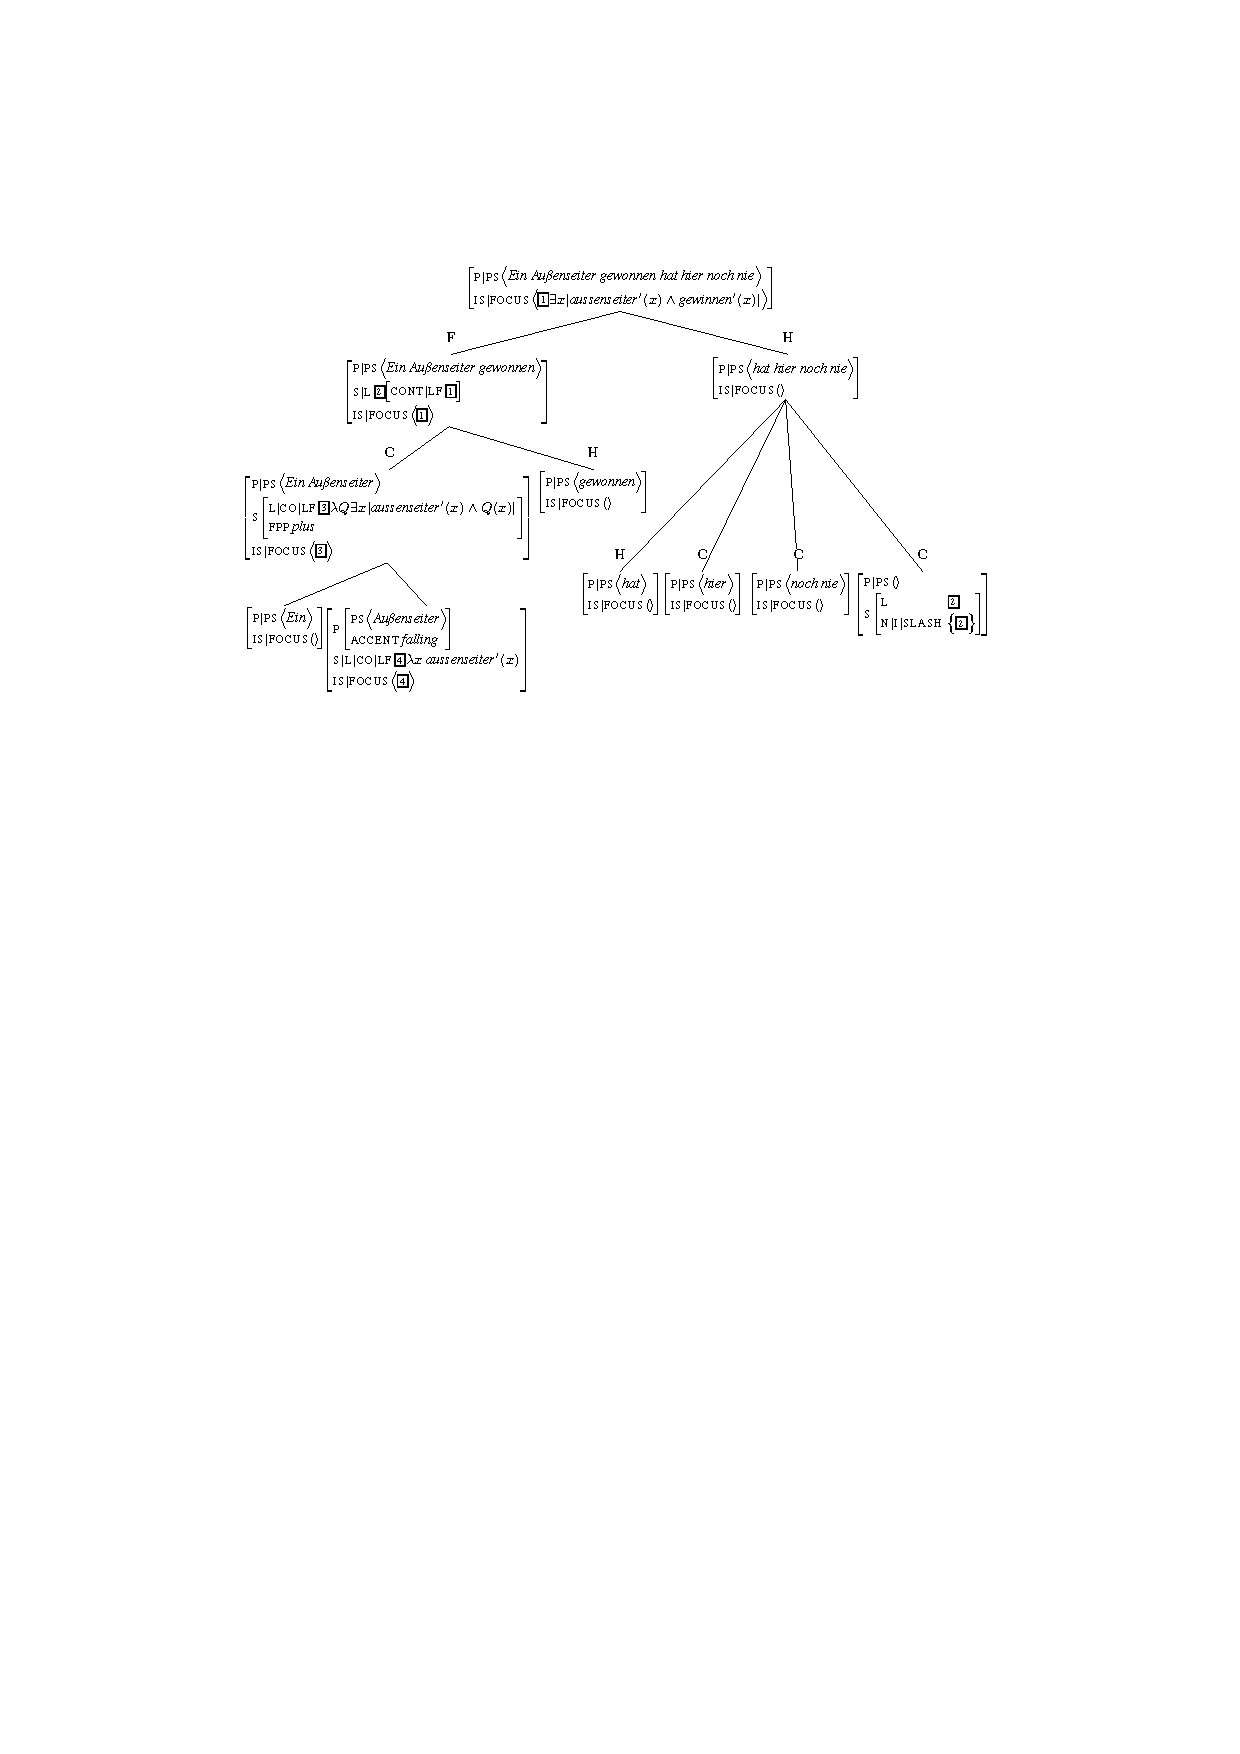
\includegraphics[scale=0.9]{figures/vp-focus-exponent}
    \caption{Partial VP fronting in \cite{dKM2003a}}
    \label{fig:focus-exponent}
  \end{figure}
  The entry of \textit{gewinnen} (to win) (the base form of the verb
  \textit{gewonnen} in example (\ref{ex:nonerg-subj-fronted}) in
  Figure~\ref{fig:lex-entry} encodes the lexical property that the
  subject of this intransitive verb has focus projection potential.
\begin{figure}[htb!]
\avmoptions{center,active}%
\begin{center}
  \begin{avm}
    [ phon & \XlstI{\phonfont{gewinnen}}\\
    arg-s & \XlstI{[fpp  \tpv{plus}\\
      loc|cat|head|case \tpv{nom}]} ]
  \end{avm}
\caption{The lexical entry of \textit{gewinnen} `to win'}
\label{fig:lex-entry}
\end{center}\unskip
\end{figure}

Under the assumption that in example (\ref{ex:nonerg-subj-fronted})
the noun \textit{Außenseiter} carries a pitch accent, the
information"=structure principle for words in~\pref{fig:words} on p.~\pageref{fig:words}
ensures that the noun contributes its \textsc{logical-form} value to
its \textsc{focus} value. The focus projection principle in~\pref{fig:focus-projection} on p.~\pageref{fig:focus-projection} ensures that the focus can project
over the entire NP \textit{ein Außenseiter}, i.e., its \textsc{focus}
element is identical to its \textsc{lf} value. Since \textit{ein
  Außenseiter} as the subject of \textit{gewonnen} in the tree in
Figure~\ref{fig:focus-exponent} is lexically marked as \textsc{fpp}
\textit{plus}, the principle governing focus projection in the verbal
domain in~\pref{fig:focus-projection} licenses the focus to
project over the entire fronted verb phrase \textit{ein
  Außenseiter gewonnen}. The fronted constituent thus contributes its
\textsc{lf} value to its \textsc{focus} value. In this example, the
focus does not project further so that in the head-filler phrase the
focus values of the two daughters are simply collected as licensed by
the first disjunct of the focus principle in~\pref{fig:focus-projection} we discussed earlier in
section~\ref{sec:struc-meaning}. As a result, the \textsc{focus} value
of the fronted verb phrase is the \textsc{focus} value of the
entire sentence. Finally, note that the example satisfies Webelhuth's
generalization, which requires a fronted verb phrase to be the
focus of the utterance as formalized in the principle in~\pref{fig:webelhuths-generalization}.

In the same spirit, \cite{BC2010a} show that sentences in which
multiple elements have been fronted \is{multiple fronting} are directly linked to specific
types of information structure. In German as a V2 language, normally
exactly one constituent occurs in the position before the finite verb
in declarative sentences. But so-called multiple fronting examples
with more than one constituent occurring before the finite verb have
been well attested in naturally occurring data \citep{Mueller2003b}. Two examples from
\cite{BC2010a} are shown in (\ref{ex:multiple-fronting}).\footnote{The examples are corpus examples that were extracted by \cite{BC2010a} from Deutsches Referenzkorpus (DeReKo), hosted at Institut für Deutsche Sprache, Mannheim: http://www.ids-mannheim.de/kl/projekte/korpora}
\begin{exe}
  \ex\label{ex:multiple-fronting}
  \begin{xlist}
    \ex\gll [Dem Saft] [eine kräftigere Farbe] geben Blutorangen.\\
             to.the juice a more.vivid colour give blood.oranges\\
      \trans `What give the jiuce a more vivid colour is blood oranges.'
    \ex\gll [Stets] [einen Lacher] [auf ihrer Seite] hatte die Bubi Ernesto Family.\\
            always a laugh on their side had the Bubi Ernesto Family\\
        \trans `Always good for a laugh was the Bubi Ernesto Family.'
  \end{xlist}

\end{exe}

But, as discussed by Bildhauer and Cook, such multiple fronting
examples seem to require very special discourse conditions in order to
be acceptable. Just like the fronted verb phrases discussed in
\cite{dKM2003a} above, \cite{BC2010a} propose
to analyze multiple fronting constructions in German as head-filler
phrases, which in this case introduce a topic shift. Following the
approach by \cite{Mueller2005d-unlinked}, multiple fronting
configurations can be identified via the filler daughter which must
have a \textsc{head|dsl} (double shlash) value of type
\textit{local}.\footnote{In Müller’s (2005) formalization, filler daughters in multiple fronting configurations (and only in these) have a  \textsc{head|dsl} value of type \textit{local}, i.e., they contain information about an empty verbal head. The \textsc{dsl} (‘double slash’) feature is needed to model the HPSG equivalent of verb movement from the sentence final position to initial position. } As introduced above, \cite{BC2010a} assume that an
information structure attribute is specified in \textit{synsem}
objects, with the features \textsc{focus} and \textsc{topic} taking
lists of \textit{elementary predications} as their values. In general,
multiple fronting \textit{head-filler} phrases are restricted by the
constraint in~\pref{fig:multiplefronting}.
\ea
Relating multiple fronting to focus \citep[75]{BC2010a}\\
  \centering
    \begin{avm}
      [\tp{head-filler-phrase}\\
      non-head-dtrs & \XlstI{[loc|cat|head|dsl & local]}]
    \end{avm}
$\to$\ 
  \begin{avm}
    [is & pres $\vee$ a-top-com $\vee$ ...]
  \end{avm}

\bigskip
    \begin{avm}
      [\tp{head-filler-phrase}\\
        is & pres]
    \end{avm}
$\to$\ 
  \begin{avm}
    [ss|loc|cat|head|dt & \XlstI{[loc|cont|rels @1]}\\
      hd-dtr|ss|is|focus & \XlstI{@1}]
  \end{avm}
  \label{fig:multiplefronting}
\z
The first constraint ensures that \textit{head-filler} phrases that
are instances of multiple frontings are restricted to have an
\textsc{is}-value of an appropriate type.\footnote{\cite[75]{BC2010a}
  assume that the type \textit{is} as the appropriate value for
  \textsc{is} has several subtypes specifying specific combinations of
  \textsc{topic} and \textsc{focus} values, such as \textit{pres} for
  presentational focus or \textit{a-top-com} for
  assessed-topic-comment.} The second constraint then ensures that in
presentational multiple frontings the designated topic of the head
daughter (i.e. the verbal head of the \textit{head-filler-phrase})
must be focused. The feature \textsc{dt} (designated topic) lexically specifies which
element, if any, is normally realized as the topic of a particular
verb. This constraint thus encodes what \cite{BC2010a} call ``topic
shift'': the non-fronted element in a multiple fronting construction
that would preferably be the topic is realized as a focus. A similar
constraint is introduced for another instance of multiple frontings,
which is called \textit{propositional assessment} multiple
fronting. Here it has to be ensured that the designated topic must be
realized as the topic somewhere in the head-daughter and the
head-daughter must also contain a focused element.

\cite{Webelhuth2007a-u} provides another account of the special
information structural requirements of fronted constituents, in this
case of predicate fronting in English that is based on the interaction
of word order and information structural constraints.
\begin{exe}
  \ex I was sure that Fido would bark and \textit{bark he did}.
\end{exe}

The principles part of Webelhuth's account require that in such cases
of predicate fronting the auxiliary is focussed and the remainder of
the sentence is in the background. The two
principles needed for this interaction are shown in~\pref{fig:predicatepreposing}.
\ea
Predicate preposing phrases \citep{Webelhuth2007a-u}:\\
  \centering
  \begin{avm}
    [\tp{aux-wd}\\
      arg-s & \XlstI{\normalfont{NP}, gap-ss}]
  \end{avm}
$\to$\ 
\begin{avm}
  [ss|status & foc\\
   arg-s & \XlstI{[status & bg], gap-ss}]
\end{avm}

\bigskip
\begin{avm}
  [\textit{pred-prepos-ph}]
$\to$\ 
\begin{avm}
  [\textit{hd-fill-ph}\\
    non-hd-dtr & [ss|status & bg]]
\end{avm}
  
\end{avm}
  \label{fig:predicatepreposing}
\z
The first constraint ensures that auxiliary words whose predicate
complement have the potential to be preposed (i.e. is of type \textit{gap-ss}) have the
information status \textit{focus}, whereas the status of the first
argument (the subject) is \textit{background}. Additional constraints
then ensure that auxiliary words with a gapped second argument can
only occur in predicate preposing phrases, and vice versa, that
predicate preposing phrases contain the right kind of auxiliary.

\section{Information structure and prosody}
\label{sec:prosody}
A lot of languages mark information structure \is{prosody} prosodically, as for
example English and German, where pitch accents of various shapes are
used to mark focus. Accordingly, several of the above discussed
approaches include a component, which enriches the phonology representation
of signs such that it allows the integration of the necessary prosodic
aspects, as for example accents.

\cite{EV96a} assume, that signs can be marked for particular accents
signalling focus or links in English, so-called A and B \isi{accents}.
In a similar way, \cite{deKuthy2002a} extends the value of
\isfeat{phon} \textsc{phon} such that it includes a feature
\isfeat{accent} \textsc{accent}, in order to formulate constraints on
the connection between accents and information structure markings.
Most of approaches discussed above do not include a detailed analysis
of the prosodic properties of the respective language that is being
investigated with respect to discourse properties. As a result, most
approaches do not go beyond the postulation of one or two particular
accents, which are then somehow encoded as part of the \textsc{phon}
value. These accents more or less serve as an illustration how lexical
principles can be formulated within a particular theory that constrain
the distribution of information structural values on the lexical
level. The more articulate such a representation of \textsc{phon}
values including accent pattern, intonation contours, boundary tone
etc is, the more detailed the principles could be that are needed to
connect information structure to prosodic patterns in languages that
signal discourse properties via intonation contours.

In \cite{Bildhauer2008a}, such a detailed account of the prosodic
properties of \ili{Spanish} is developed together with a proposal how to
integrate prosodic aspects into the \textsc{phon} value, also allowing
a direct linking of the interaction of prosody and information
structure.  In his account, the representation of \textsc{phon} values
in HPSG is enriched to include four levels of prosodic constituency,
i.e., phonological utterance, intonational phrases, phonological
phrases and prosodic words. The lowest level, prosodic words of type
\textit{pwrd}, include the feature \textsc{segs}, which corresponds to
the original \textsc{phon} value assumed in HPSG, and additional
features such as \textsc{pa} for pith accents or \textsc{bd} for
boundary tones, to encode whether a boundary tone is realized on that
word. The additional features \textsc{ut} (phonological utterance),
\textsc{ip} (intonational phrase) and \textsc{php} (phonological phrase)
encode via the typ \textit{epr} (edges and prominence) which role
a prosodic word plays in higher level constituents. For example, the
feature \textsc{dte} (designated terminal element) specifies, whether
the word is the most prominent one in a phonological phrase. A sign's
\textsc{phon} list then contains all \textit{pwrd} objects and
relational constraints define the role each prosodic word plays in
the higher prosodic constituents. This flat representation of prosodic
constituency still allows to express constraints about intonational
contours associated with certain utterance types. One example
discussed in Bildhauer's work is the contour associated with broad
focus declaratives in \ili{Spanish}, which can be decomposed into a
sequence of late-rise (L*H) prenuclear accents, followed by an
early-rise nuclear accent (LH*), followed by a low boundary tone
(L\%). The constraint introduced to model this contour for declarative
utterances thus instantiates the \textsc{bd} value (boundary tone) of
the last \textit{pwrd} (prosodic word) in the \textsc{phon} list to low, instantiates
a nuclear pitch accent \textit{low-high-star} on this rightmost
prosodic word and ensures that a prenuclear pitch accent
\textit{low-star-high} is instantiated on every preceding compatible
prosodic word. The constraint encoding this is shown in~\pref{fig:spanish-intonation}.
\ea
Intonational contour of Spanish declarative utterances \citep[142]{Bildhauer2008a}:\\
%  \centering
  \begin{tabular}[t]{l@{  }r@{}l@{}}
  \begin{avm}
    \normalfont{\textit{decl-tune(@1)}}\end{avm} & $\leftrightarrow$ & \begin{avm} @1 = @2 $\oplus$ \<[pa & low-high-star\\
                                                                  bd & low]\> \end{avm}
$\wedge$\\
& &
\begin{avm}
  @2 = \normalfont{\textit{list}}([bd & none])
\end{avm}
$\wedge$\\
& &
\begin{avm}
@2 = \normalfont{\textit{list}}([pa & none]) $\shuffle$ \normalfont{\textit{list}}([pa & low-star-high])\end{avm}
\\[4ex]
\begin{avm}
[\normalfont{\textit{sign}}\\
  embed & $-$]\end{avm} & $\rightarrow$ & \begin{avm} [phon @1] $\wedge$ \normalfont{\textit{decl-tune}}(@1)
  \end{avm}  \\
  \end{tabular}
\label{fig:spanish-intonation}
\z
The second constraint in~\pref{fig:spanish-intonation} ensures
that only unembedded utterances can be constrained to the just
described declarative tune. That this specific contour is then
compatible with a broad focus reading is ensured by an additional
principle expressing a general focus prominence constraint for
\ili{Spanish}, namely that focus prominence has to fall on the last prosodic
word in the phonological focus domain, which, in the case of a broad
focus, can be the entire utterance. The principle formulated in Bildhauer's account is shown in~\pref{fig:focus-prominence}.
\ea
Focus prominence in Spanish \citep[146]{Bildhauer2008a}:\\
  \centering
  \begin{avm}
    [\tp{sign}\\
       cont & @1\\
       foc & @1]
\ $\rightarrow$\
[phon \normalfont{\textit{list}} $\oplus$ <[ut|dte & $+$]>]
  \end{avm}

  \label{fig:focus-prominence}
\z
Since only words
that are the designated terminal element (\textsc{dte}) can bear a
pitch accent, the interplay of the two principles above ensures, that
in utterances with a declarative contour the entire phrase can be in
the focus. These principles thus nicely illustrate, how not only
lexical elements can contribute to the information structure via their
prosodic properties, but how entire phrases with specific prosodic
properties can be constrained to have specific information structural
properties.

The approach of \cite{song2018} also includes a component that
captures the interaction between prosodic properties of utterances and
the effect on the information structure. In order to include
information structural constraints of the so-called A and B accents in
English, several components of Bildhauer's (2007) phonological
architecture are adapted for the information structural set up in
\cite{song2018}. Among them is the idea that in a phonological phrase
(encoded in the feature phonological utterance \textsc{ut}) focus
prominence is related to the most prominent word in that phrase, which
is encoded via the constraint in~\pref{ex:song-mkg}.
\ea
\label{ex:song-mkg}
Prosodic marking of focus \citep[159]{song2018}\\
\begin{avm}
 \normalfont{\textit{lex-rule}} $\rightarrow$\  [ut|dte & @1\\mkg|fc & @1]
\end{avm}
\z
Specific lexical principle for the A and B accent then ensure the
correct information structural marking and specifiy which type of
element has to be present on the \textsc{icons} list. The
specification necessary for English A accents signalling focus (here characterized as
\textit{high-star}) are shown
in~\pref{ex:song-a-accent}.
\ea
\label{ex:song-a-accent}
Focus marking of A accents in English \citep[160]{song2018}\\
\textit{fc-lex-rule} $\rightarrow$
\begin{avm}
  [ut|dte & $+$\\
  pa & high-star\\
  mkg & fc-only\\
  index & @1\\
  incons-key & @2\\
  c-cont|icons &  \<\ \normalfont{!} @2[\tp{semantic-focus}\\target @1]\ \normalfont{!}\ \> \\
  dtr|head & +nv]
\end{avm}
\z

\section{Conclusion}
\label{sec:conclusion}

We have discussed various possibilities of how to represent
information structure within HPSG's sign-based architecture.
Several approaches from the HPSG literature were presented which all
have in common that they introduce a separate feature
\textsc{info"=struc} into the HPSG setup, but they differ in (i) where
they locate such a feature, (ii) what the appropriate values are for
the representation of information structure, and (iii) how they encode
principles constraining the distribution and interaction of
information structure with other levels of the grammatical
architecture. Finally, we discussed a number of theories in which
phenomena such as word order are constrained to be only well-formed in
case they exhibit specific information structural properties.

%  {\sloppy
%  \printbibliography[heading=subbibliography,notkeyword=this] }


\printbibliography[heading=subbibliography,notkeyword=this] 
\end{document}

%%% Local Variables: 
%%% coding: utf-8
%%% mode: latex
%%% TeX-engine: xetex
%%% TeX-master: "../main.tex"
%%% End: 
